\mcchap{Le dashboard}{cap:dashboard}

\noindent La dashboard è stata realizzata utilizzando Dash, un framework Python ideato per costruzione di applicazioni web di analytics.
Dash si appoggia a Flask, Plotly.js e react.js. Dash ideale per la costruzione di applicazioni di visualizzazione dati con elevata personalizzazione in puro Python. E’ particolarmente indicato per chiunque lavori con i dati in Python.

\begin{figure}[htp]
    \centering
    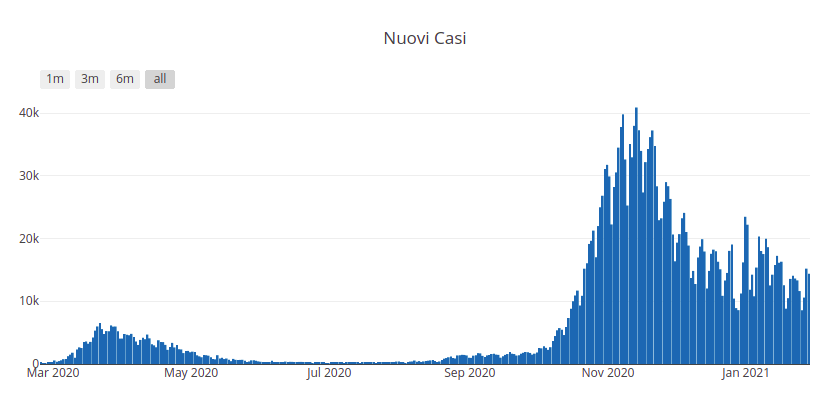
\includegraphics[width=9cm]{new_cases}
    \caption{Esempio grafico - nuovi casi}
    \label{fig:chart_example}
\end{figure}

\section{Dashboard italia}
La dashboard Italiana contiene i seguenti grafici
\begin{itemize}
    \item Nuovi Casi
    \item Totale Casi
    \item Isolamento domiciliare
    \item Terapia intensiva
    \item Nuovi casi normalizzati
    \item Terapia intensiva e Ospedalizzati
    \item Media a 7 giorni dei decessi giornalieri e contagi
    \item Percentuale nuovi positivi sui casi testati
    \item Nuovi casi vs nuovi decessi
\end{itemize}


\section{Dashboard Lombardia}

\section{Dashboard Regioni}

